\documentclass{sig-alternate}
\usepackage{url}
\usepackage{graphicx}
\usepackage{subfigure}
\usepackage{hyperref}
\usepackage{url}
\usepackage{times}
\usepackage{balance}
\usepackage{xspace}
\usepackage{paralist}
\usepackage{relsize}

%\usepackage{xfrac}

\begin{document}

\newcommand{\todo}[1]{\textbf{TODO}\footnote{\textbf{TODO:} #1}}

\newcommand{\ghtorrent}{\textsc{ght}orrent\xspace}
\newcommand{\api}{\textsc{api}\xspace}
\newcommand{\pullreqs}{\textsf{pullreqs}\xspace}

\title{A Dataset for Pull Request Research}
\numberofauthors{2}

\author{
\alignauthor
Georgios Gousios\\
       \affaddr{Delft University of Technology}\\
       \affaddr{Delft, the Netherlands}\\
       \email{g.gousios@tudelft.nl}
\and
Andy Zaidman\\
       \affaddr{Delft University of Technology}\\
       \affaddr{Delft, the Netherlands}\\
       \email{a.e.zaidman@tudelft.nl}
}

\maketitle

\begin{abstract}

Pull requests form a new method for collaborating in distributed software
development. To study the pull request distributed development model, we
constructed a dataset of almost 900 projects and 350,000 pull requests, 
including some of the largest
users of pull requests on Github. In this paper, we describe how the project
selection was done, we analyze the selected features and present a machine
learning tool set for the R statistics environment. 

\end{abstract}

\category{D.2.7}{Software Engineering}{Distribution, Maintenance, and Enhancement}[Version control]
\category{D.2.9}{Software Engineering}{Management}[Programming teams]

\terms{Management}

\keywords{pull-based development, pull request, distributed software development,
empirical software engineering}

\section{Introduction}
\label{sec:intro}

Pull requests as a distributed development model in general, and as implemented
by Github in particular, form a new method for collaborating on distributed
software development. In the pull-based development model, the project's main
repository is not shared among potential contributors; instead, contributors
\emph{fork} (clone) the repository and make their changes independent of each
other. When a set of changes is ready to be submitted to the main repository,
they create a pull request, which specifies a local branch to be merged with a
branch in the main repository. A member of the project's core team is then
responsible to inspect the changes and pull them to the project's master branch.
If changes are considered unsatisfactory, more changes may be requested; in that
case, contributors need to update their local branches with new commits.
Furthermore, as pull requests only specify branches from which certain commits
can be pulled, there is nothing that forbids their use in the shared 
repository approach (cross-branch pull requests).

To understand what the underlying principles that guide pull-based development
are, we created \pullreqs, a curated dataset of almost 900 projects along with a
set of tools for its analysis. A previous version of the dataset has been used
to quantitatively study the pull request development process~\cite{GPD14}. The
\pullreqs dataset is based on our previous work on \ghtorrent~\cite{Gousi13},
albeit only for its construction. While \ghtorrent is a full mirror of all
data offered by the Github {\sc api}, the \pullreqs dataset includes many features extracted by combining \ghtorrent and the project's repository; the dataset is offered in a format ready to be processed by statistical software.
In this paper, we describe the construction
process of the dataset and outline directions for further research with it.

\section{Feature Selection}
\label{sec:expdata}

The feature selection was based on prior work in the areas of patch submission
and acceptance~\cite{Nagap05,Bird07a,Weiss08,Baysa12}, code
reviewing~\cite{Rigby13}, bug triaging~\cite{Anvik06, Giger10} and also
on semi-structured interviews of Github developers~\cite{Dabbi12, Pham13}. The
selected features are split into three categories:

  \emph{Pull request characteristics.} These features attempt to quantify the
  impact of the pull request on the affected code base. When examining external
  code contributions, the size of the patch is affecting both acceptance and
  acceptance time~\cite{Weiss08}. There are various metrics to determine the
  size of a patch that have been used by researchers: code churn~\cite{Nagap05},
  changed files~\cite{Nagap05} and number of commits.
  In the particular case of pull requests, developers reported that the presence
  of tests in a pull request increases their confidence to merge
  it~\cite{Pham13}. To investigate this, we split the churn feature into two
  features, namely \texttt{src\_churn} and \texttt{test\_churn}. The
  number of participants has been shown to influence the time to process of code
  reviewing~\cite{Rigby13}. Finally, through our own experience analyzing pull
  requests, we have found that in many cases conflicts are reported explicitly
  in pull request comments while in other cases pull requests include links to
  other related pull requests.

  \emph{Project characteristics.} These features quantify how receptive to pull
  requests the project is. If the project's process is open to external
  contributions, then we expect to see an increased ratio of external
  contributors over team members. The project's size may be a detrimental factor
  to the speed of processing a pull request, as its impact may be more difficult
  to assess. Also, incoming changes tend to cluster over time (the ``yesterday's
  weather'' change pattern), so it is natural to assume that pull
  requests affecting a part of the system that is under active development will
  be more likely to merge. Testing plays a role in speed of processing;
  according to~\cite{Pham13}, projects struggling with a constant flux of
  contributors use testing, manual or preferably automated, as a safety net to
  handle contributions from unknown developers.

  \emph{Developer.}  Developer-based features quantify the influence that the
  person who created the pull request has on the decision to merge it and the
  time to process it. In particular, the developer who created the patch has
  been shown to influence the patch acceptance decision~\cite{Jeong09}. To
  abstract the results across projects with different developers, we include
  features that quantify the developer's track record~\cite{Dabbi12}, namely the
  number of previous pull requests and their acceptance rate; the former has
  been identified as a strong indicator of pull request quality~\cite{Pham13}.
  Bird et al.~\cite{Bird07}, presented evidence that social reputation has an
  impact on whether a patch will be merged; in our dataset, the number of
  followers on Github can be seen as a proxy for reputation.



All features must be calculated at the time a pull request has been closed or
merged, to evaluate the effect of intermediate updates to the pull request as a
result of the ensuing discussion. Features that contain a temporal dimension in
their calculation (e.g., \texttt{team\_size} or
\texttt{commits\_on\_files\_touched}) are calculated over the three-month time
period before the pull request was opened.

\section{Dataset Construction}

The distribution of pull requests per project in Github is extremely skewed
(quantiles 5\%: 1, 95\%: 68, mean: 26, median: 4). By the end of 2013, 255,914
projects had received a pull request while only 8,600 had received more than
100. To ensure that the selected projects used pull requests as part of the
project development cycle, rather than just occasional external contributions,
we only selected the top 1\% of projects by total number of pull requests
created. The initial selection led to 2,551 projects.
In addition, to evaluate testing related features as described above,
we needed a way to determine whether a source code file in a project
repository represented test code.
For that, we exploited the
convention-based project layout in the Ruby (Gem), Python, Java and Scala (both
Maven) language ecosystems, so our project selection was limited to those
languages. 1,517 projects where thus filtered out.

For the remaining 1,034 repositories, the full history (including pull requests,
issues and commits) of the included projects was downloaded and features were
extracted by querying the \ghtorrent databases and analyzing each project's Git
repository.

\begin{figure}
  \begin{center}
    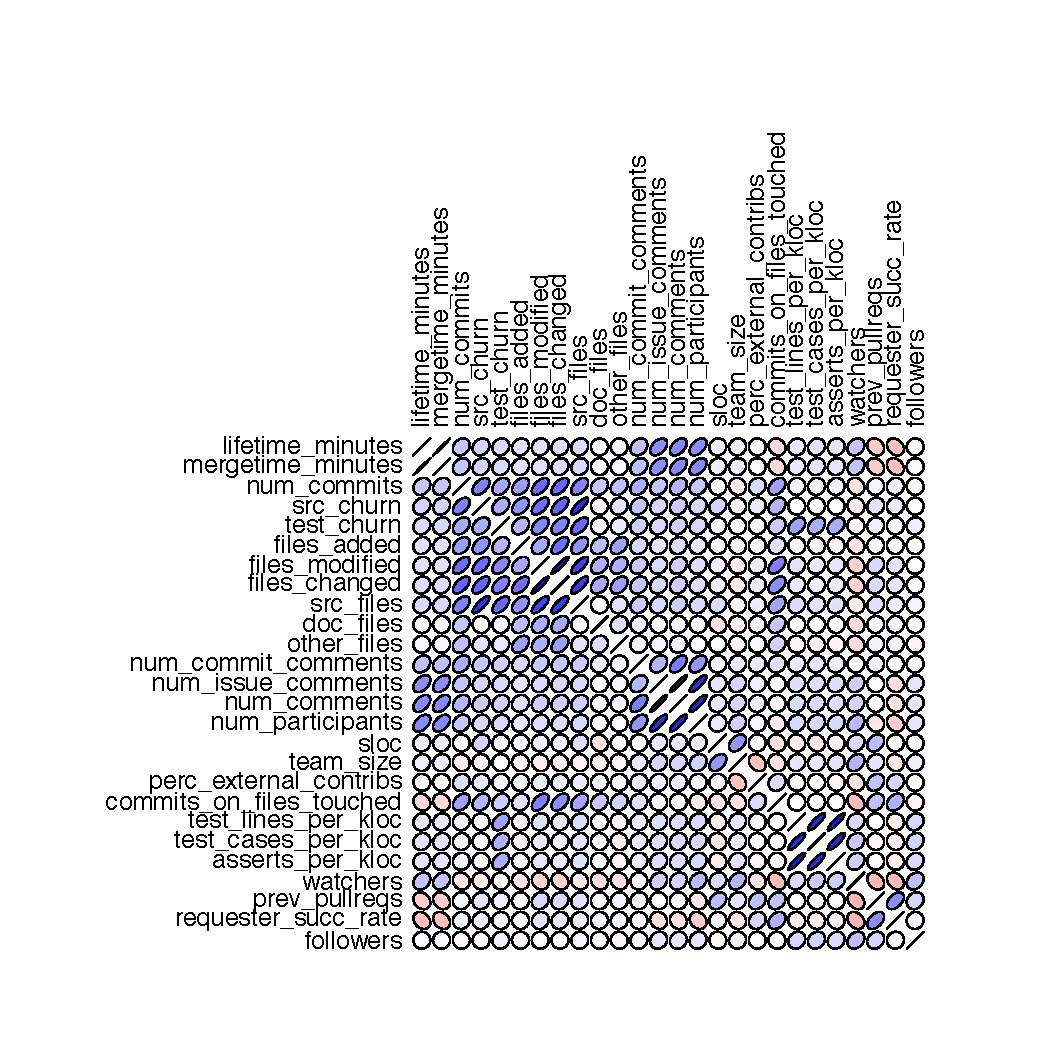
\includegraphics[scale=0.6]{cross-cor.pdf}
  \end{center}
  \caption{Cross-correlation (Spearman) among all dataset features. Blue color (or right slant) indicates positive correlation, red color (or left slant) is negative correlation. The darker the color, the stronger the correlation.}
  \label{fig:features}
\end{figure}

% latex table generated in R 2.15.3 by xtable 1.7-1 package
% Sat Jan 11 16:56:59 2014
\begin{table*}
\centering
\begin{tabular}{rp{20em}rrrrc}
  \hline
  \bfseries{Feature} & \bfseries{Description} & \bfseries{5\%} & \bfseries{mean} & \bfseries{median} & \bfseries{95\%} & \bfseries{histogram} \\ 
  \hline
   \multicolumn{2}{l}{\bf{Pull Request Characteristics}}\\
lifetime\_minutes & Minutes between opening and closing & 0.00 & 15,418 & 581.00 & 72,508 & 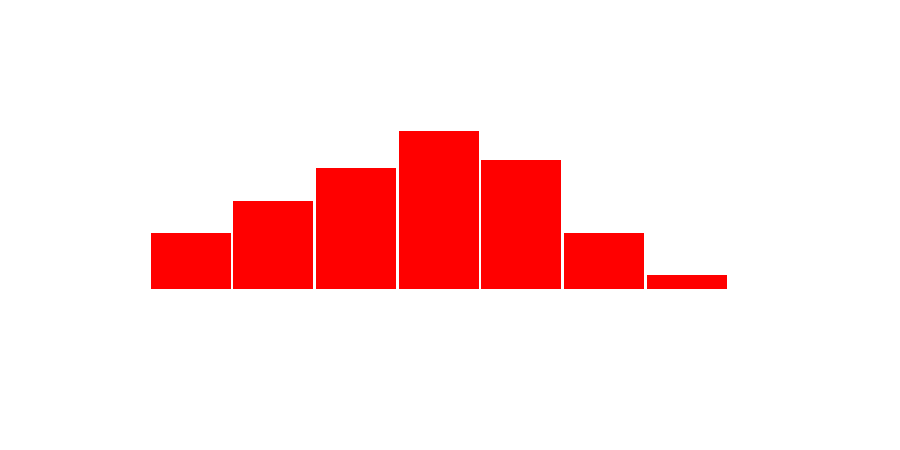
\includegraphics[scale = 0.1, clip = true, trim= 50px 60px 50px 60px]{hist-29b6fa715eecc1dad108c8148465533b.pdf} \\ 
  mergetime\_minutes & Minutes between opening and merging (only for merged pull
    requests) & 0.00 & 10,506 & 418.00 & 44,234 & 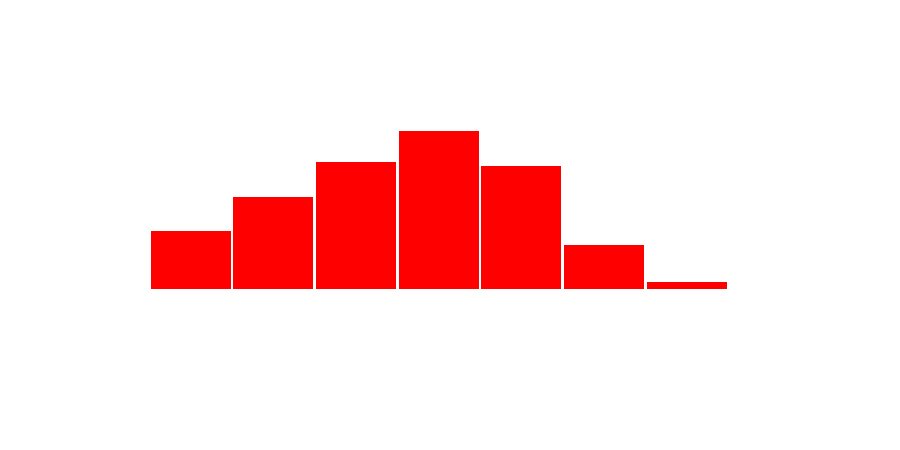
\includegraphics[scale = 0.1, clip = true, trim= 50px 60px 50px 60px]{hist-e2ded77f4080f561e112a1f363b125ce.pdf} \\ 
  num\_commits & Number of commits & 1.00 & 4.42 & 1.00 & 12.00 & 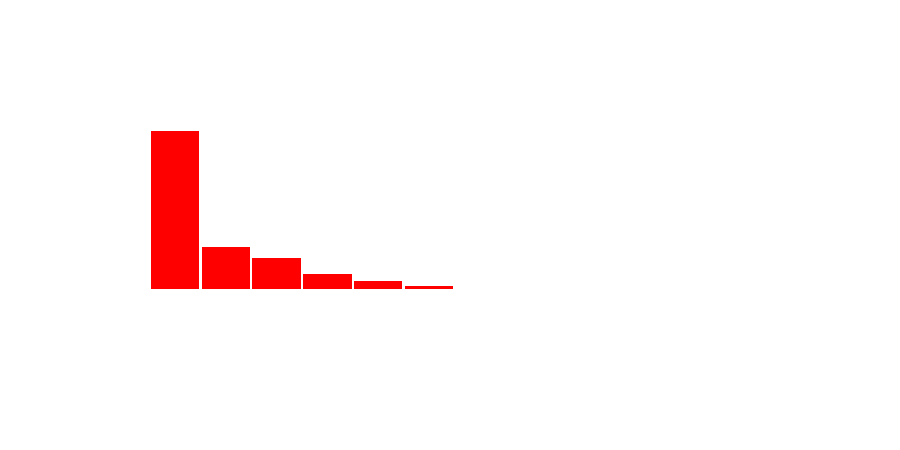
\includegraphics[scale = 0.1, clip = true, trim= 50px 60px 50px 60px]{hist-f128f3cb38588fe5202716588c047381.pdf} \\ 
  src\_churn & Number of lines changed (added + deleted) & 0.00 & 282.95 & 10.00 & 846.00 & 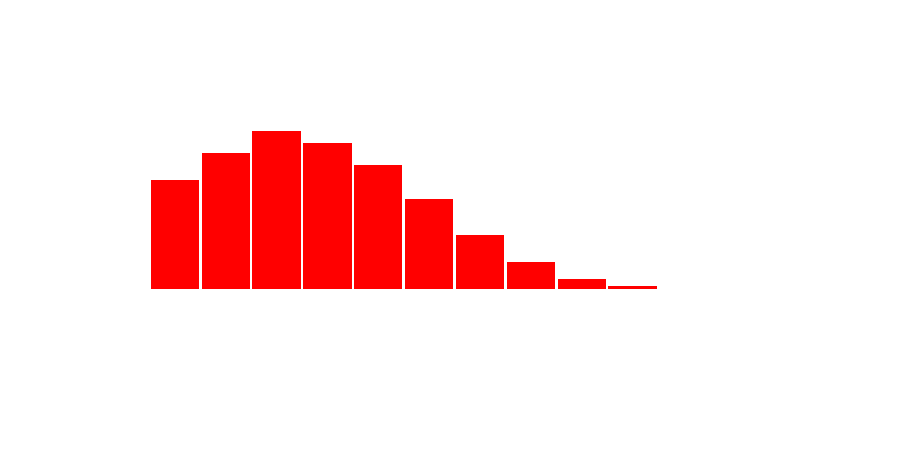
\includegraphics[scale = 0.1, clip = true, trim= 50px 60px 50px 60px]{hist-1f006c80a0da61518435a0c55f538326.pdf} \\ 
  test\_churn & Number of test lines changed & 0.00 & 79.74 & 0.00 & 248.00 & 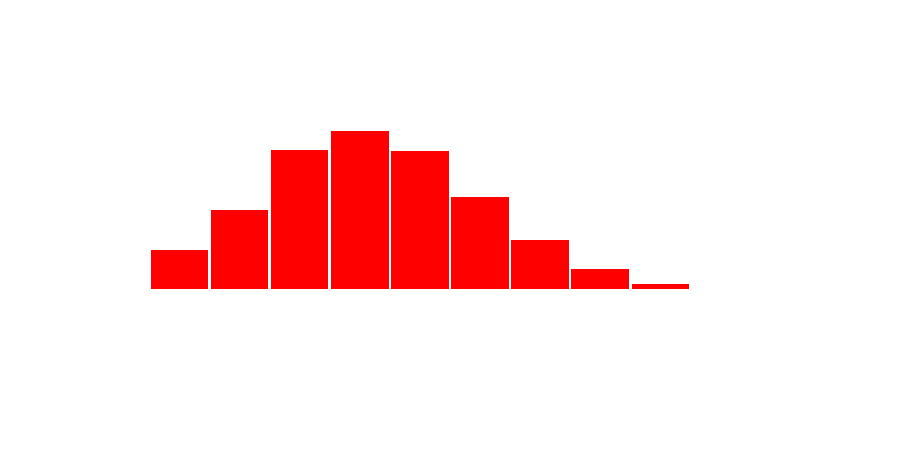
\includegraphics[scale = 0.1, clip = true, trim= 50px 60px 50px 60px]{hist-dd78ccaeedd7fc79735a66eb7f9e506b.pdf} \\ 
  files\_added & Number of files added  & 0.00 & 4.01 & 0.00 & 7.00 & 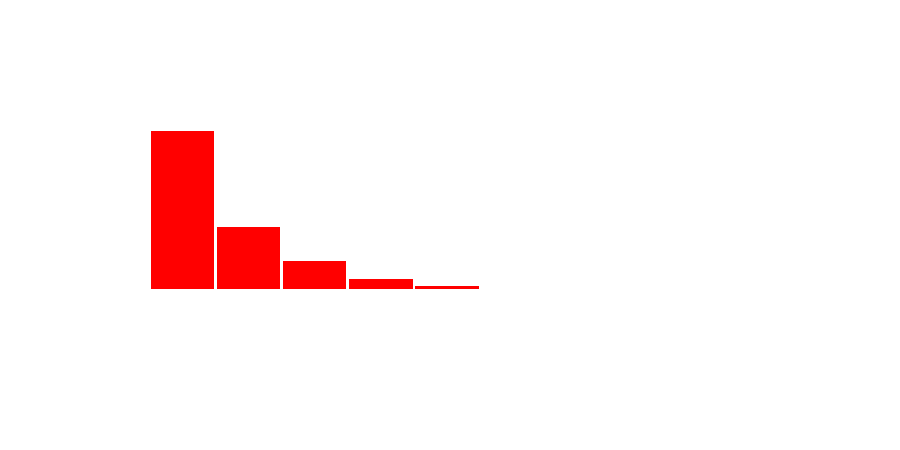
\includegraphics[scale = 0.1, clip = true, trim= 50px 60px 50px 60px]{hist-340be33adc9a51666460c68028842c1d.pdf} \\ 
  files\_deleted & Number of files deleted  & 0.00 & 2.05 & 0.00 & 1.00 & \includegraphics[scale = 0.1, clip = true, trim= 50px 60px 50px 60px]{hist-bd564691a0c6275ea5f30bcc0b81b3f5.pdf} \\ 
  files\_modified & Number of files modified  & 1.00 & 7.56 & 2.00 & 21.00 & 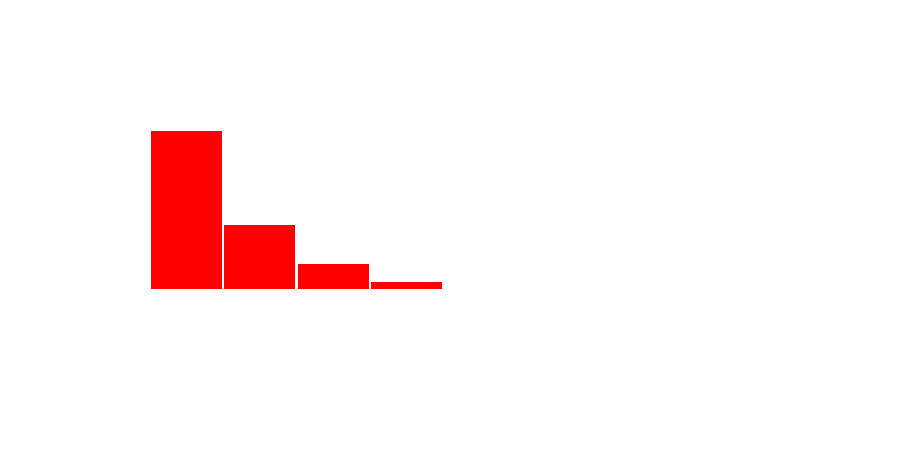
\includegraphics[scale = 0.1, clip = true, trim= 50px 60px 50px 60px]{hist-52a19dc5ca5e4f8c5325bca43137a6c1.pdf} \\ 
  files\_changed & Number of files touched (sum of the above) & 1.00 & 13.62 & 2.00 & 32.00 & 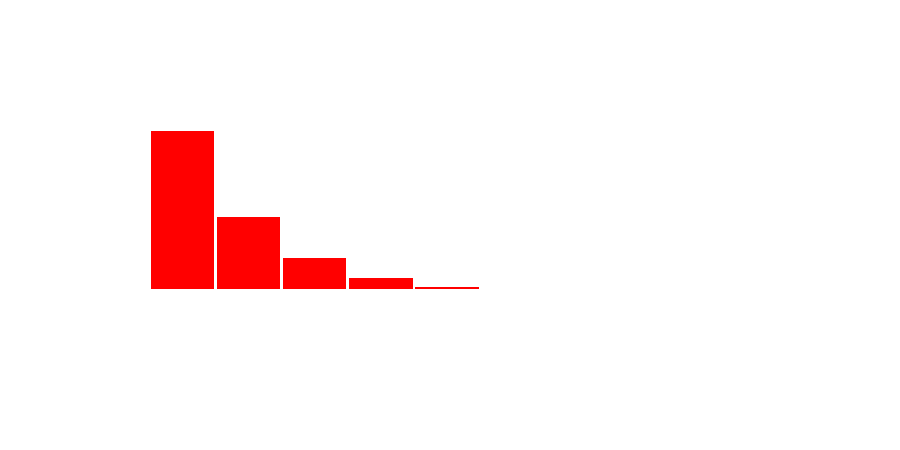
\includegraphics[scale = 0.1, clip = true, trim= 50px 60px 50px 60px]{hist-9b07b060359435635ff2bf4cd34f834a.pdf} \\ 
  src\_files & Number of source code files touched by the pull request & 0.00 & 7.64 & 1.00 & 20.00 & 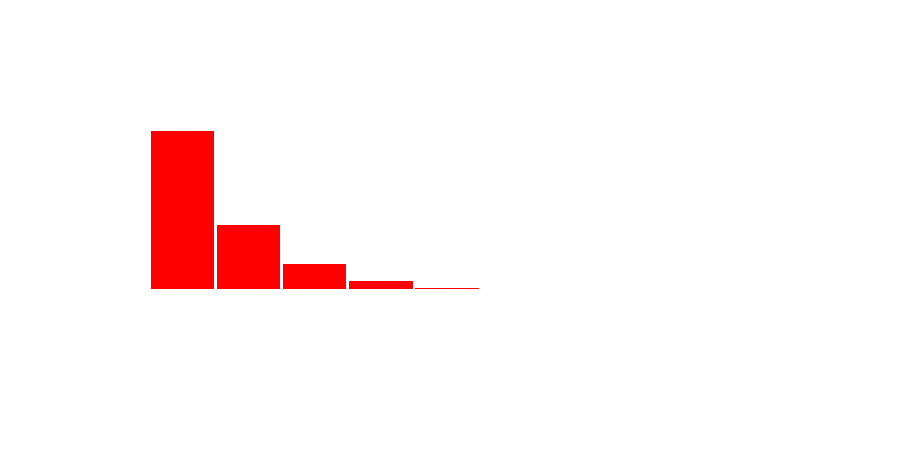
\includegraphics[scale = 0.1, clip = true, trim= 50px 60px 50px 60px]{hist-2d4e53ba8eec29c0c79c1e834756c654.pdf} \\ 
  doc\_files & Number of documentation (markup) files touched & 0.00 & 2.36 & 0.00 & 6.00 & 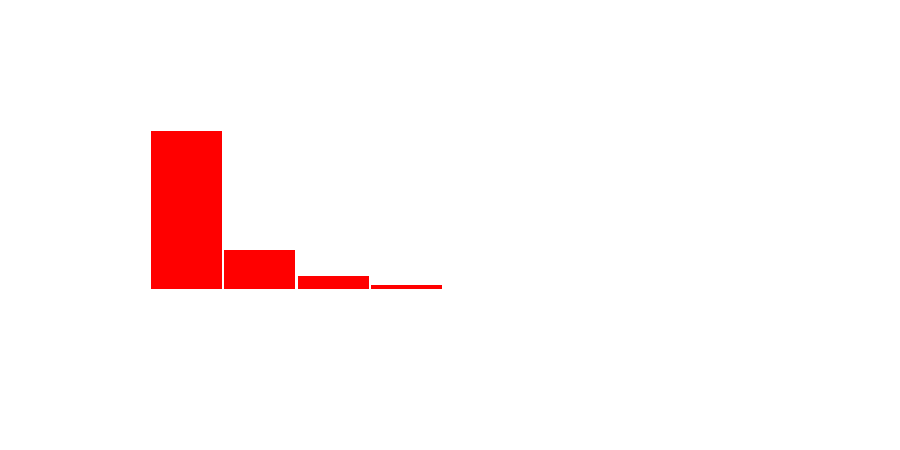
\includegraphics[scale = 0.1, clip = true, trim= 50px 60px 50px 60px]{hist-d4fb585969e7acb86dd568d80e7f1500.pdf} \\ 
  other\_files & Number of non-source, non-documentation files touched & 0.00 & 2.74 & 0.00 & 4.00 & 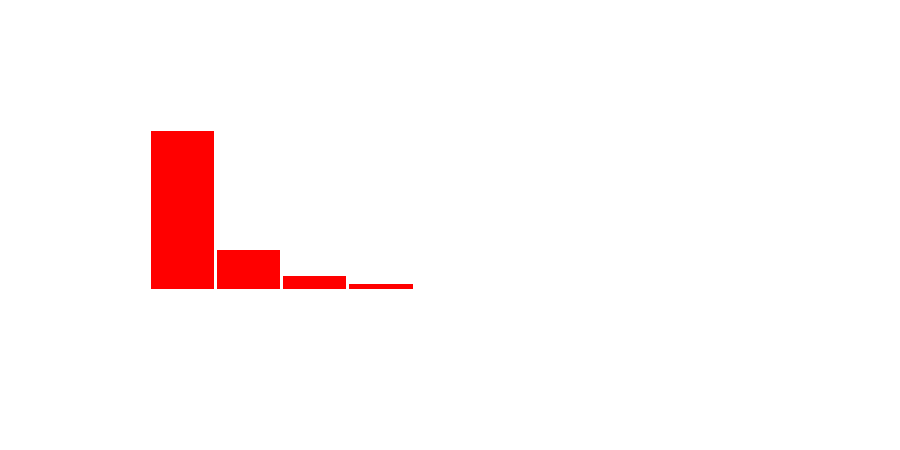
\includegraphics[scale = 0.1, clip = true, trim= 50px 60px 50px 60px]{hist-df965fcd0b03a96f1b31b2eda13d2b98.pdf} \\ 
  num\_commit\_comments & The total number of code review comments & 0.00 & 0.73 & 0.00 & 4.00 & 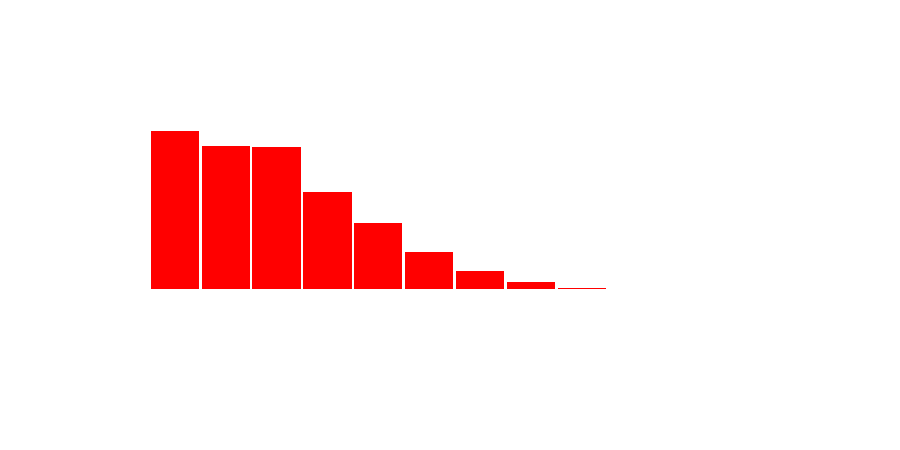
\includegraphics[scale = 0.1, clip = true, trim= 50px 60px 50px 60px]{hist-f0fac61db5a83629be8f04cc84e8b907.pdf} \\ 
  num\_issue\_comments & The total number of discussion comments & 0.00 & 1.84 & 0.00 & 8.00 & 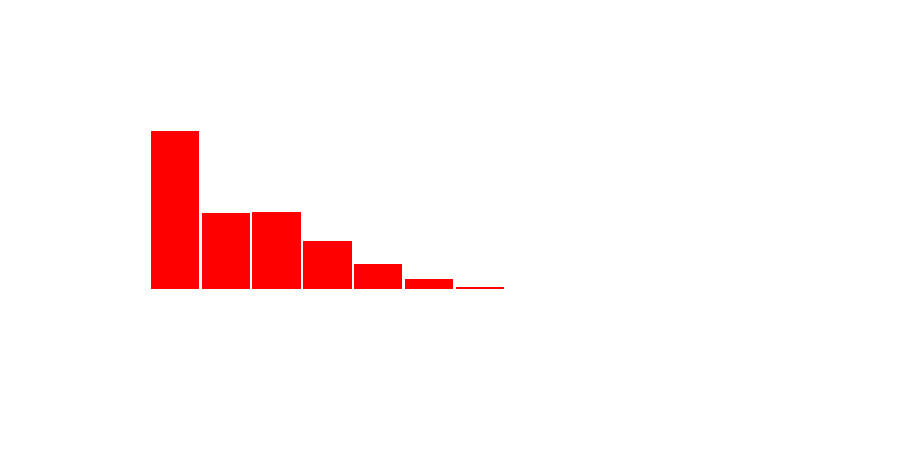
\includegraphics[scale = 0.1, clip = true, trim= 50px 60px 50px 60px]{hist-fee6653ed7b2359f7e7374841378492b.pdf} \\ 
  num\_comments & The total number of comments (discussion and code review). & 0.00 & 2.57 & 1.00 & 11.00 & 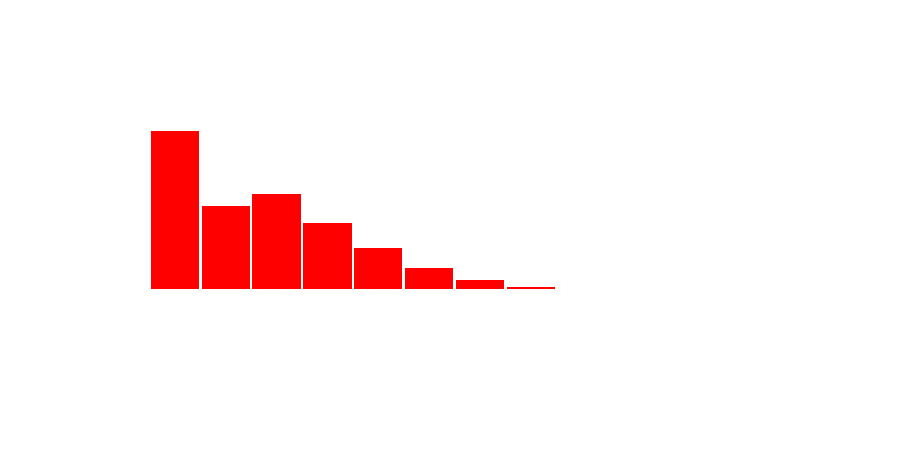
\includegraphics[scale = 0.1, clip = true, trim= 50px 60px 50px 60px]{hist-9db5e2b390de0d64d26c14798cb579ef.pdf} \\ 
  num\_participants & Number of participants in the discussion & 0.00 & 1.27 & 1.00 & 4.00 & 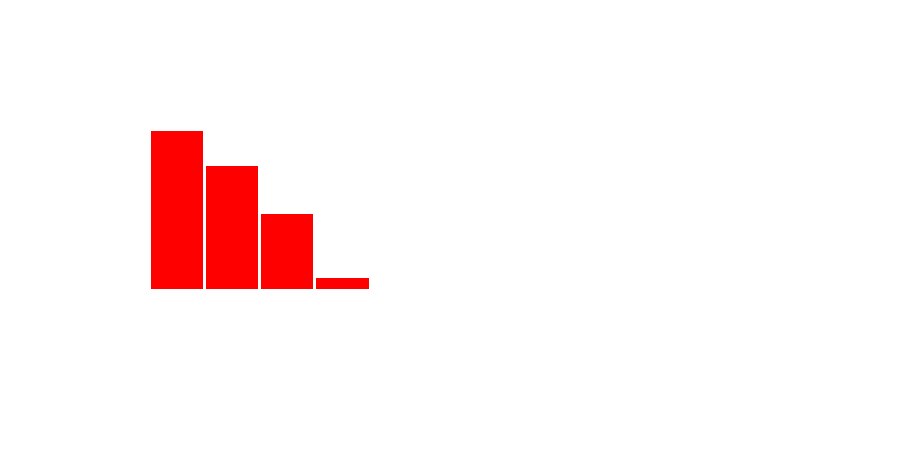
\includegraphics[scale = 0.1, clip = true, trim= 50px 60px 50px 60px]{hist-7d419bb69f175ea7015a9bdc71172f38.pdf} \\ 
  \multicolumn{2}{l}{\bf{Project Characteristics}}\\
  
  sloc & Executable lines of code at creation time. & 458.00 & 53,801 & 18,019 & 275,058 & 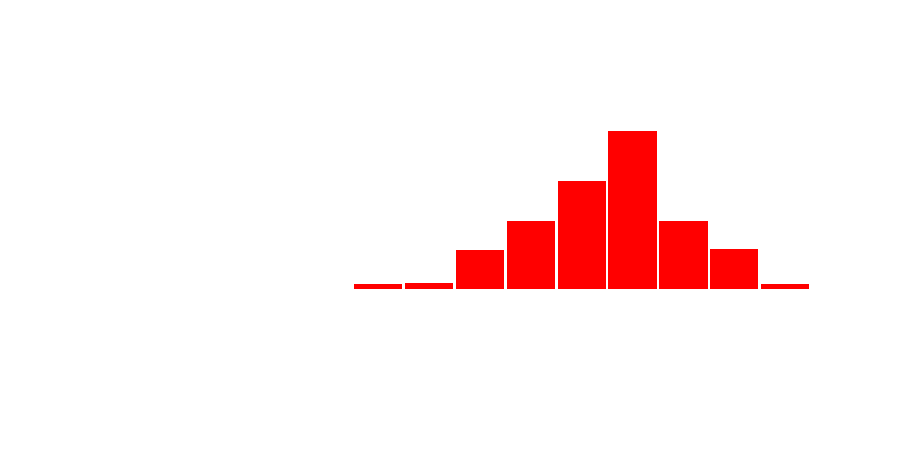
\includegraphics[scale = 0.1, clip = true, trim= 50px 60px 50px 60px]{hist-6b5159d3060b4fdf8493d4c818f79949.pdf} \\ 
  team\_size & Number of active core team members during the last 3 months prior to creation. & 1.00 & 20.64 & 7.00 & 93.00 & 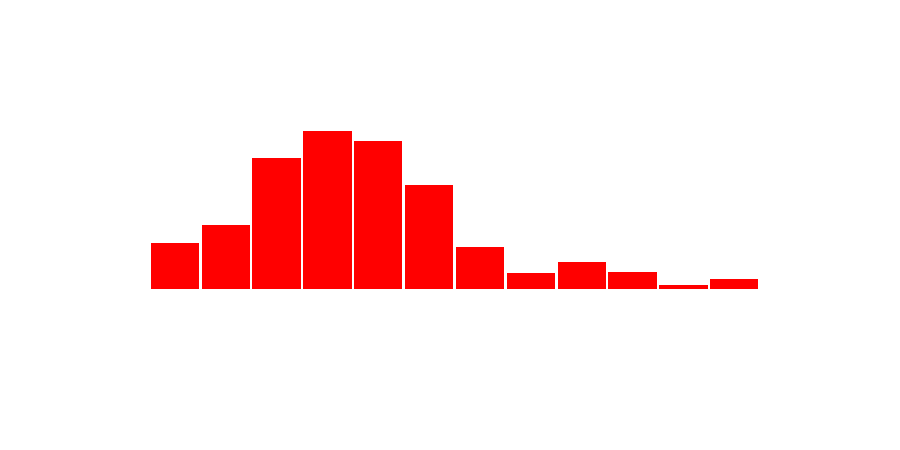
\includegraphics[scale = 0.1, clip = true, trim= 50px 60px 50px 60px]{hist-231fb4fabf4a3f0c551f2a97ae080508.pdf} \\ 
  perc\_external\_contribs & The ratio of commits from external members over core team members in the last 3 months prior to creation. & 8.00 & 54.01 & 56.00 & 95.00 & 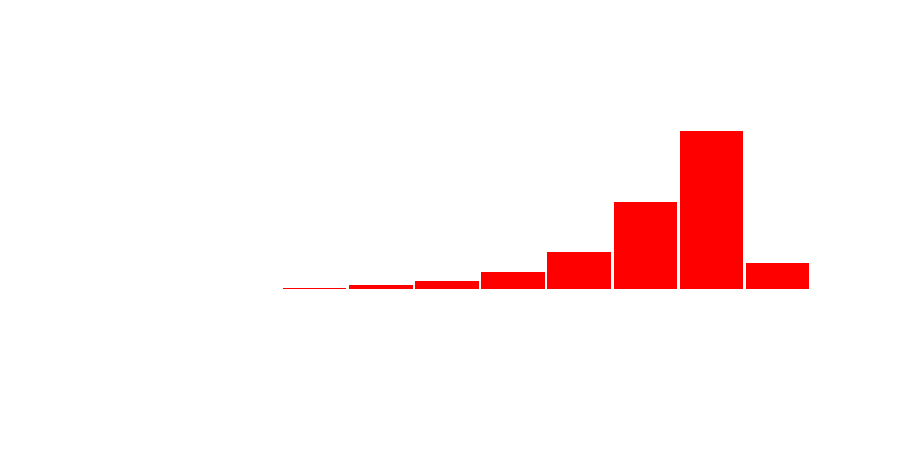
\includegraphics[scale = 0.1, clip = true, trim= 50px 60px 50px 60px]{hist-a222f0a5c377ba129dd6c8f257062591.pdf} \\ 
  commits\_on\_files\_touched & Number of total commits on files touched by the pull request 3 months before the creation time. & 0.00 & 51.65 & 4.00 & 209.00 & 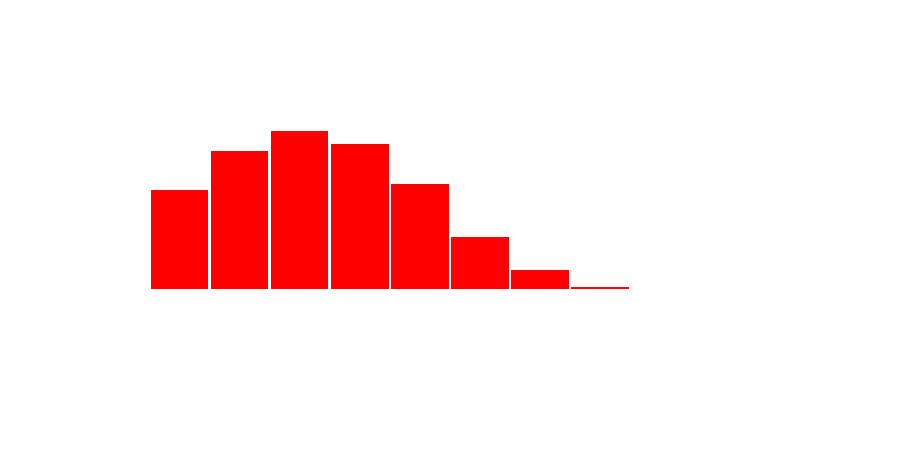
\includegraphics[scale = 0.1, clip = true, trim= 50px 60px 50px 60px]{hist-b735900ffcc37e7eda16dcd0c3497e6e.pdf} \\ 
  test\_lines\_per\_kloc & Executable lines of test code per 1,000 lines of source code & 0.00 & 1,297 & 355.21 & 2,097 & 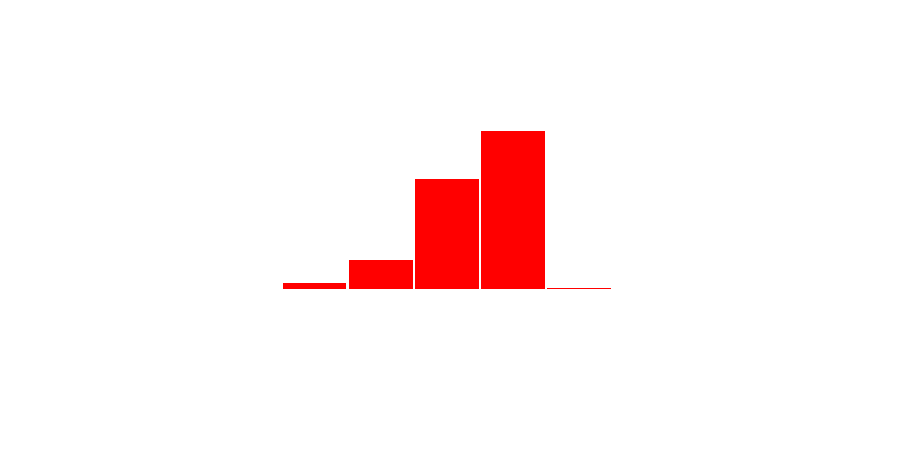
\includegraphics[scale = 0.1, clip = true, trim= 50px 60px 50px 60px]{hist-67ff3047089ba9ce0528884eab66e80a.pdf} \\ 
  test\_cases\_per\_kloc & Number of test cases per 1,000 lines of source code & 0.00 & 83.74 & 14.55 & 181.03 & 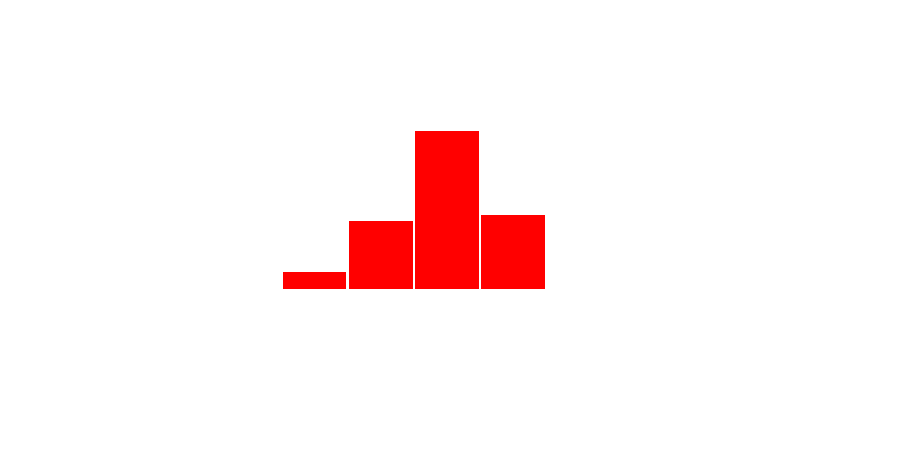
\includegraphics[scale = 0.1, clip = true, trim= 50px 60px 50px 60px]{hist-2b62bb5f7ccb31fe66208a895c8dd549.pdf} \\ 
  asserts\_per\_kloc & Number of assert statements per 1,000 lines of source code & 0.00 & 200.30 & 40.37 & 479.11 & 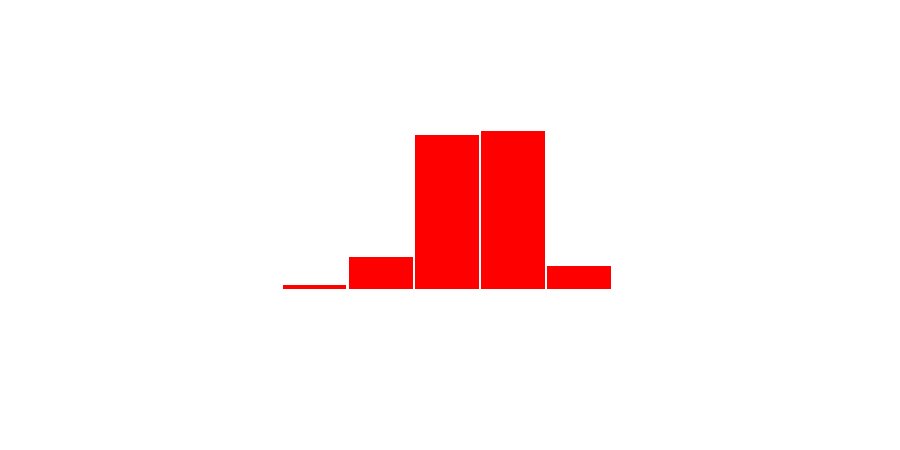
\includegraphics[scale = 0.1, clip = true, trim= 50px 60px 50px 60px]{hist-4ad84a89acf32483001ce11c881622b8.pdf} \\ 
  watchers & Project watchers (stars) at creation & 4.00 & 1,778 & 310.00 & 11,114 & 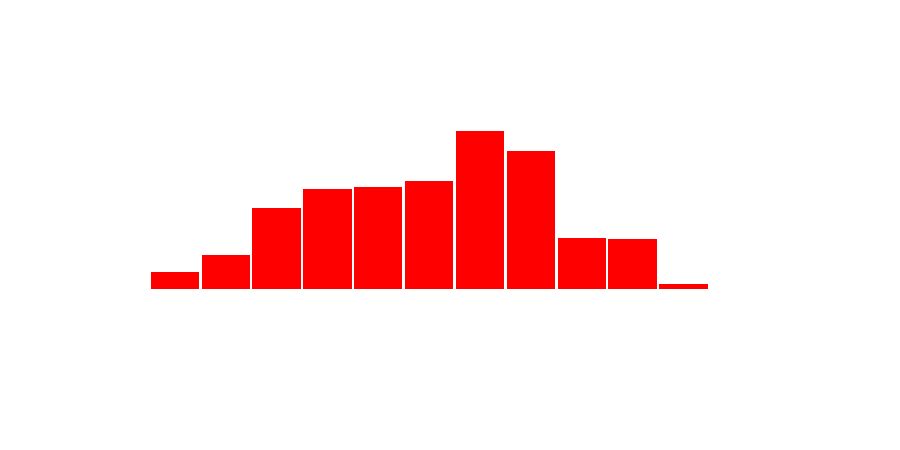
\includegraphics[scale = 0.1, clip = true, trim= 50px 60px 50px 60px]{hist-d097a7d1786ca9917e46e0fda1adb365.pdf} \\

  \multicolumn{2}{l}{\bf{Developer Characteristics}}\\
  
  prev\_pullreqs & Number of pull requests submitted by a specific developer, prior to the examined one & 0.00 & 42.81 & 11.00 & 196.00 & 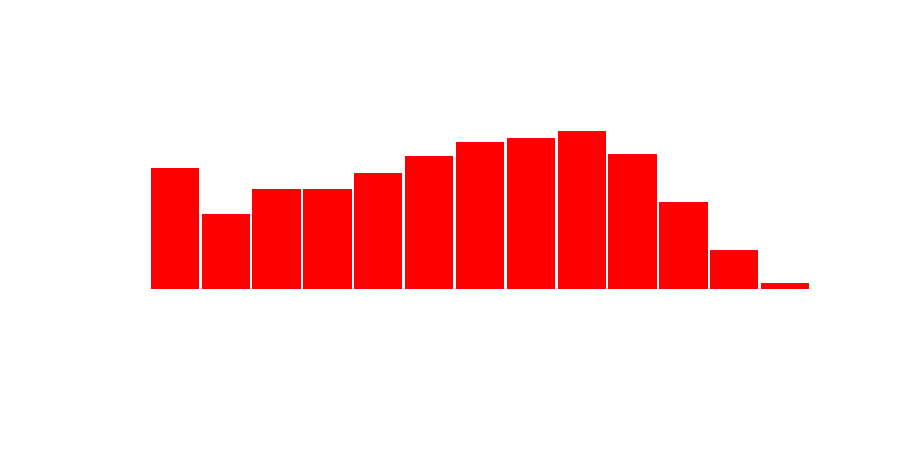
\includegraphics[scale = 0.1, clip = true, trim= 50px 60px 50px 60px]{hist-a2f7f60851dfa13cfbe0227d1d233767.pdf} \\ 
  requester\_succ\_rate & The percentage of the developer's pull requests that have been merged up to the creation of the examined one & 0.00 & 0.51 & 0.62 & 1.00 & 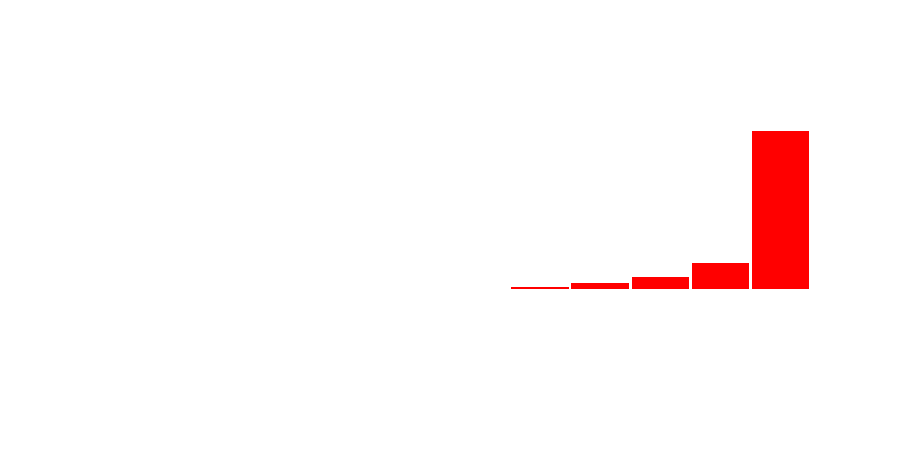
\includegraphics[scale = 0.1, clip = true, trim= 50px 60px 50px 60px]{hist-9363017165c3ded62457750f1c67c1af.pdf} \\ 
  followers & Followers to the developer at creation & 0.00 & 20.93 & 4.00 & 80.00 & 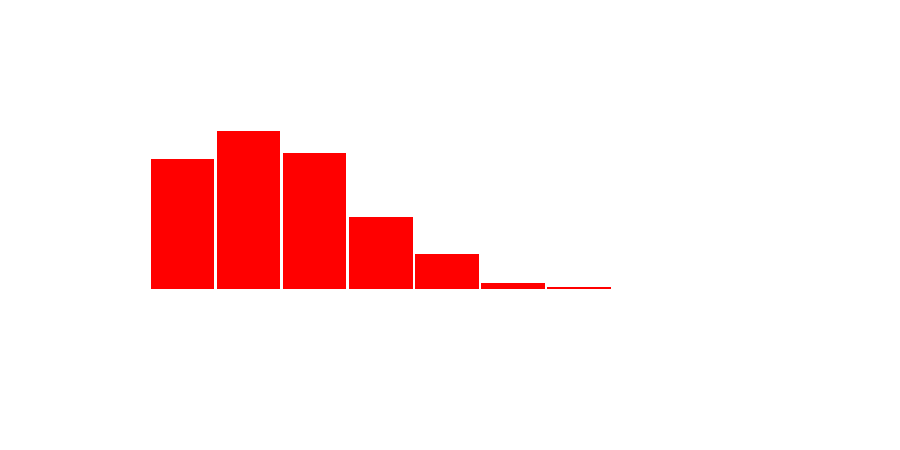
\includegraphics[scale = 0.1, clip = true, trim= 50px 60px 50px 60px]{hist-a7f2f738f15a09420e70e9a2c30e2aef.pdf} \\ 
   \hline
\end{tabular}
\caption{Selected features and descriptive statistics. A data point is a pull request. Historgrams are in log scale.} 
\label{tab:features}
\end{table*}


\paragraph*{Merge detection}
To identify pull requests that are merged outside Github, we resorted to
the following heuristics, listed here in order of application:

\begin{compactdesc}

  \item[$H_1$] At least one of the commits associated with the pull request appears in the target project's master branch.

  \item[$H_2$] A commit closes the pull request (using the \texttt{fixes:}
    convention advocated by Github) and that commit appears in the project's
    master branch.  This means that the pull request commits were squashed onto
    one commit and this commit was merged.

  \item[$H_3$] One of the last 3 (in order of appearance) discussion comments
    contain a commit unique identifier, this commit appears in the project's
    master branch and the corresponding comment can be matched by the following
    regular expression:

    \begin{small}
    \texttt{(?:merg|appl|pull|push|integrat)(?:ing|i?ed)}
    \end{small}

  \item[$H_4$] The latest comment prior to closing the pull request matches the
    regular expression above.

\end{compactdesc}

If none of the above heuristics identifies a merge, the pull request is
identified as unmerged.

\paragraph*{Test case detection}
In \emph{Ruby} projects, files under the \texttt{/test/} and \texttt{/spec/}
directories are considered test files. Test cases are recognized by scanning
through the test files lines for method name patterns as required by the
\textsf{RUnit}, \textsf{Rspec}, \textsf{Shoulda} and \textsf{Minitest}
frameworks. The popular Cucumber behaviour driven development testing framework
is excluded from the analysis due to inexistent naming conventions.  In
\emph{Python}, project conventions do not specify specific directories for test
files, so test file detection is based solely on whether the file name contains
the word ``test'' as prefix or suffix. Test cases and asserts are discovered
both in source code and also in API examples embedded in documentation comments. 

Following Maven conventions, in \emph{Java} projects, files in directories under
a \texttt{test/} branch of the file tree are considered test files.
\textsf{junit4} test cases are recognized using the \texttt{@Test} tag. For
\textsf{junit3}, methods starting with test are considered as test methods.
Asserts are counted by searching through the source code lines for
\texttt{assert} statements. Finally, as Maven underlies \emph{Scala}'s default
build system (\textsf{sbt}), the same conventions as in the Java case can be
used to discover test files. In addition to \textsf{junit}, the process can
discover test cases and assert statements as defined by the \textsf{scalatest}
and \textsf{specs2} testing frameworks.


\paragraph*{Counting lines, files and file types}

In the \pullreqs dataset, a line of code is an executable statement,
excluding blank lines and comments. To measure lines, we developed custom
comment strippers for all the programming languages the dataset supports, as
we could not find any tool that can count lines reliably (block comments in Ruby and Python were a particular problem).
Moreover, we delegated the identification of file types to a Ruby library
called Linguist (the same that Github uses), which supports more than 250 file types.

\paragraph*{Further Quality Control}
After the dataset was constructed, the following criteria were applied to 
ensure homogeneity:

\begin{compactitem}

  \item After processing, the number of remaining pull requests should be more
    that 90\% of the initially calculated number of pull requests.
    The typical reason for some pull requests missing from the output
    is that many projects use a dedicated branch for documentation which
    includes no source code; the data generation script skips such pull
    requests. Other reasons might include the project has beed deleted from
    Github or no source code files could be identified in a specific version. 
    38 projects were filtered out.

  \item Projects should have at least one commit coming from a developer outside
    the project's main team, to ensure that the project is open to external
    contributions and that pull requests are not just used by developers within
    the project. No projects were excluded due to this criterion. 

  \item The ratio of merged pull requests should be within reasonable limits
    from the mean merge ratio across all Github projects. In the \ghtorrent
    dataset, the mean merge ratio is 72\%. The \pullreqs dataset uses heuristics
    to identify merges done outside Github, so we generally expect a mean merge
    ratio close to or higher of the one across Github.

\end{compactitem}

\paragraph*{Results} The final dataset consists of 895 projects (302 Python, 252 Java, 304 Ruby, 37
Scala) and 332,643 pull requests (115,703; 84,156; 115,703 and 18,691for Python,
Ruby, Java and Scala projects respectively). 58\% of the pull requests are
merged using Github's facilities while 18\% are identified as unmerged.
The remaining 24\% is identified as merged using the heuristics described
above ($H_1$: 10\%, $H_2$: 4\%, $H_3$: 3\%, $H_4$: 7\%).
Moreover, as Figure~\ref{fig:features} shows,
the selected features are fairly orthogonal, with very few strong correlations
between them. This indicates that they capture a wide range of pull
request activities with minimal overlap.

\section{Tools}

The \pullreqs dataset is accompanied by an extensive analysis toolkit written in
the R statistics language. The framework allows researchers to load selections
of projects in R, provides basic statistics in tabular (e.g.
Table~\ref{tab:features}) and graphical form (e.g. Figure~\ref{fig:features}),
and exposes a command line base interface that tools can extend. Moreover,
it implements a modular, multi-step data mining framework that researchers
can easily re-use in similar machine learning experiments. The data mining
parts include all the necessary steps for successfully executing a data mining
experiment, such as distribution plotting, cross correlation among features,
pluggable model and algorithm definitions, $n$-fold cross-validation and
plotting of important model variables such as Area Under Curve ({\sc auc}) and
accuracy across cross-validation runs. To cope with the \pullreqs dataset
size, several parts of the tooling employ parallelism and can thus exploit
multi-core machines.

\section{Related Work}
\label{sec:rel}

The \pullreqs dataset is similar to the code review datasets published by
Hamasaki et al.~\cite{Hamas13} and Mukadam et al.~\cite{Mukad13}.  It improves
upon those two datasets by covering a wider array of projects and languages
while also offering more precise related data, such as file counts and test
cases. To the best of our knowledge, this is the only publicly available
dataset covering pull-based development and certain aspects of distributed
software development in general.

\section{Research Opportunities and Conclusion}

The \pullreqs dataset can be used for a multitude of studies, apart from
basic exploration of the pull-based distributed development model.

We presented the \pullreqs dataset, a curated dataset of almost 900 projects,
along with a statistical analysis tool set for its analysis. New research directions whose analysis can be facilitated
by this dataset can include code review activities, recommender systems for pull
request handling and triaging and investigation of project process openness. The
dataset itself can be extended to support more programming languages and more
projects. Pull requests are especially welcome!

All source code and data is available on the Github repository
\href{https://github.com/gousiosg/pullreqs}{gousiosg/pullreqs}. Data on the
\href{http://ghtorrent.org}{ghtorrent.org} web site permit full replication
of the construction process or the expansion of this dataset.

\bibliographystyle{abbrv}
\balance
%\begin{small}

  \bibliography{dataset}
%\end{small}

\end{document}
